\hypertarget{the-hills-are-alive-with-the-sound}{%
\section{The hills are alive with the
sound\ldots{}}\label{the-hills-are-alive-with-the-sound}}

\begin{figure}[!ht]
  \begin{adjustwidth}{-\oddsidemargin-1in}{-\rightmargin}
    \centering
    
\includegraphics[trim={0 5cm 0 2cm,}, clip, width=\paperwidth]{./S01/img/22/the-hills-are-alive.png}
    % \caption{The Hills Are Alive\label{fig:the-hills-are-alive}}
  \end{adjustwidth}
\end{figure}

\textbf{\emph{\ldots of music}}. A galera está tirando sarro da maneira
que Chandler fala, enfatizando certas palavras, e Ross faz referência a
canção \emph{The Hills Are Alive} do filme \emph{The Sound of Music}
(1965) (já citado no episódio
\textbf{\textcolor{primarycolor}{Aquele onde Tudo começou}}).\footnote{\sloppy The Sound of Music | ``The Hills Are Alive'' Lyric Video | Fox Family Entertainment. \url{https://www.youtube.com/watch?v=yvQ4t-Nk128}}

\hypertarget{joan-collins}{%
\section{Joan Collins}\label{joan-collins}}

\begin{figure}[!ht]
  \begin{adjustwidth}{-\oddsidemargin-1in}{-\rightmargin}
    \centering
    
\includegraphics[trim={0 5cm 0 2cm,}, clip, width=\paperwidth]{./S01/img/22/joan-collins.png}
    % \caption{Joan Collins\label{fig:joan-collins}}
  \end{adjustwidth}
\end{figure}

\begin{tcolorbox}[enhanced,center upper,
    drop fuzzy shadow southeast, boxrule=0.3pt,
    lower separated=false, breakable,
    colframe=black!30!dialogoBorder,colback=white]
\begin{minipage}[c]{0.16\linewidth}
  \raisebox{\dimexpr-\height+\ht\strutbox\relax}{
    \centering 
\includegraphics[width=1.4cm]{./assets/img/monica.png}
  }
   & \centering \scriptsize{Monica}
\end{minipage}
\hfill
\begin{minipage}[c]{0.8\linewidth}
  \textbf{- I'm Joan Collins.}\\
  - Eu sou Joan Collins.
\end{minipage}
\end{tcolorbox}

\saveparinfos
\noindent
\begin{minipage}[c]{0.5\textwidth}\useparinfo

Monica se envolve com um rapaz bem mais novo, Ethan, e menciona
\emph{Joan Collins} (1933-), atriz inglesa famosa pelo seu papel como
\emph{Alexis Carrington} na série de TV \emph{Dynasty}
(1981-1989).\footnote{\sloppy Joan Collins - Encyclopædia Britannica. \url{https://www.britannica.com/biography/Joan-Collins}}
Na trama ela se casa com um rapaz mais novo, como parte de um esquema
para se vingar do ex-marido.

\end{minipage}\hfill
\begin{minipage}[c]{0.5\textwidth}

\begin{figure}
  \centering
  \begin{tikzpicture}
    \node [inner sep=0pt] at (0,0) {
      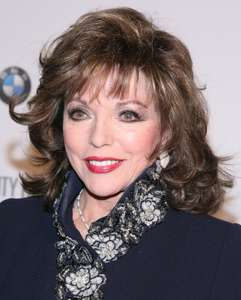
\includegraphics[width=0.7\textwidth,keepaspectratio]{./S01/img/22/joan-collins-2009.jpg}
    };
    \draw [white, rounded corners=\ClipSep, line width=\ClipSep]
    (current bounding box.north west) --
    (current bounding box.north east) --
    (current bounding box.south east) --
    (current bounding box.south west) -- cycle
    ;
    \end{tikzpicture}
    \caption{Joan Collins\label{fig:joan-collins}}
\end{figure}

\end{minipage}

\hypertarget{power-rangers}{%
\section{Power Rangers}\label{power-rangers}}

\begin{figure}[!ht]
  \begin{adjustwidth}{-\oddsidemargin-1in}{-\rightmargin}
    \centering
    
\includegraphics[trim={0 5cm 0 2cm,}, clip, width=\paperwidth]{./S01/img/22/power-rangers.png}
    % \caption{Power Rangers\label{fig:power-rangers}}
  \end{adjustwidth}
\end{figure}

\begin{tcolorbox}[enhanced,center upper,
    drop fuzzy shadow southeast, boxrule=0.3pt,
    lower separated=false, breakable,
    colframe=black!30!dialogoBorder,colback=white]
\begin{minipage}[c]{0.16\linewidth}
  \raisebox{\dimexpr-\height+\ht\strutbox\relax}{
    \centering 
\includegraphics[width=1.4cm]{./assets/img/joey.png}
  }
   & \centering \scriptsize{Joey}
\end{minipage}
\hfill
\begin{minipage}[c]{0.8\linewidth}
  \textbf{- ...could you ask him which one the strongest Power Ranger is?}\\
  - ...pergunta a ele qual o Power Ranger mais forte?
\end{minipage}
\end{tcolorbox}

A galera descobre que Ethan é menor de idade e eles provocam Monica.
Joey faz menção a série de TV \emph{Power Rangers} (1993-). Na época do
episódio de \emph{Friends} a série estava em sua segunda temporada. Na
história, seis estudantes do ensino médio, assim como Ethan, são
escolhidos pelo ser intergalático \emph{Zordon} e ganham super poderes
para combater \emph{Lord Zedd} e salvar o planeta Terra.\footnote{\sloppy Mighty Morphin Power Rangers - Website. \url{https://powerrangers.hasbro.com/pt-br/tv-shows}}

\saveparinfos
\noindent
\begin{minipage}[c]{0.45\textwidth}\useparinfo

Um detalhe interessante é que \emph{na hora de morfar}, Joey menciona
\emph{Stegosaurus}, que não faz parte dos seis animais que representam
cada personagem.

\end{minipage}\hfill
\begin{minipage}[c]{0.55\textwidth}

\begin{figure}
  \centering
  \begin{tikzpicture}
    \node [inner sep=0pt] at (0,0) {
      
\includegraphics[width=0.8\textwidth,keepaspectratio]{./S01/img/22/power-rangers-pose.jpeg}
    };
    \draw [white, rounded corners=\ClipSep, line width=\ClipSep]
    (current bounding box.north west) --
    (current bounding box.north east) --
    (current bounding box.south east) --
    (current bounding box.south west) -- cycle
    ;
    \end{tikzpicture}
    \caption{Mighty Morphin Power Rangers\label{fig:mighty-morphin-power-rangers}}
\end{figure}

\end{minipage}

\hypertarget{aux-buttes-chaumont}{%
\section{Aux Buttes Chaumont}\label{aux-buttes-chaumont}}

\begin{figure}[!ht]
  \begin{adjustwidth}{-\oddsidemargin-1in}{-\rightmargin}
    \centering
    
\includegraphics[trim={0 8cm 0 0cm,}, clip, width=\paperwidth]{./S01/img/22/aux-buttes-chaumont.png}
    % \caption{Aux Buttes Chaumont\label{fig:aux-buttes-chaumont}}
  \end{adjustwidth}
\end{figure}

O apartamento de Monica possui pôsteres emblemáticos, entre eles está o
\emph{Aux Buttes Chaumont: jouets et objets pour étrennes} (1885) do
ilustrador francês \emph{Jules Chéret} (1836-1932). Ele anunciava uma
famosa loja de brinquedos Parisiense.\footnote{\sloppy Aux Buttes Chaumont - Gallica (Francês). \url{https://gallica.bnf.fr/ark:/12148/btv1b90105877}}
O texto traduzido seria \emph{Aux Buttes Chaumont: Brinquedos e
presentes para o Ano Novo}.

\begin{figure}
  \centering
  \begin{tikzpicture}
    \node [inner sep=0pt] at (0,0) {
      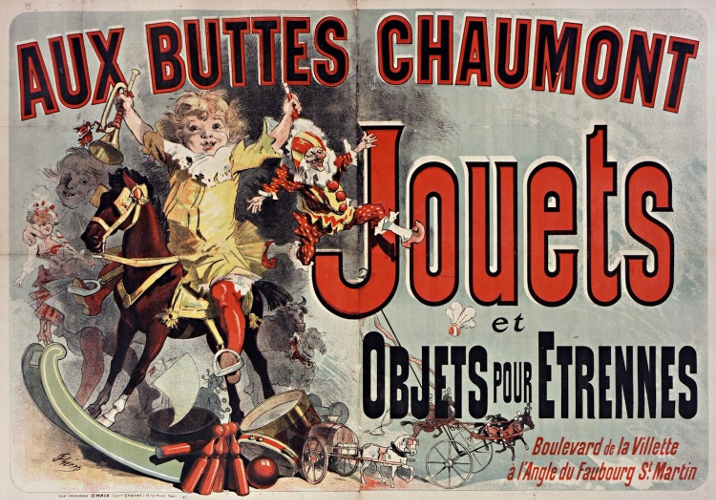
\includegraphics[width=0.6\textwidth,keepaspectratio]{./S01/img/22/aux-buttes-chaumont-poster.jpeg}
    };
    \draw [white, rounded corners=\ClipSep, line width=\ClipSep]
    (current bounding box.north west) --
    (current bounding box.north east) --
    (current bounding box.south east) --
    (current bounding box.south west) -- cycle
    ;
    \end{tikzpicture}
    \caption{Aux Buttes Chaumont - Poster\label{fig:aux-buttes-chaumont-poster}}
\end{figure}

\hypertarget{ebony-and-ivory}{%
\section{Ebony and Ivory}\label{ebony-and-ivory}}

\begin{figure}[!ht]
  \begin{adjustwidth}{-\oddsidemargin-1in}{-\rightmargin}
    \centering
    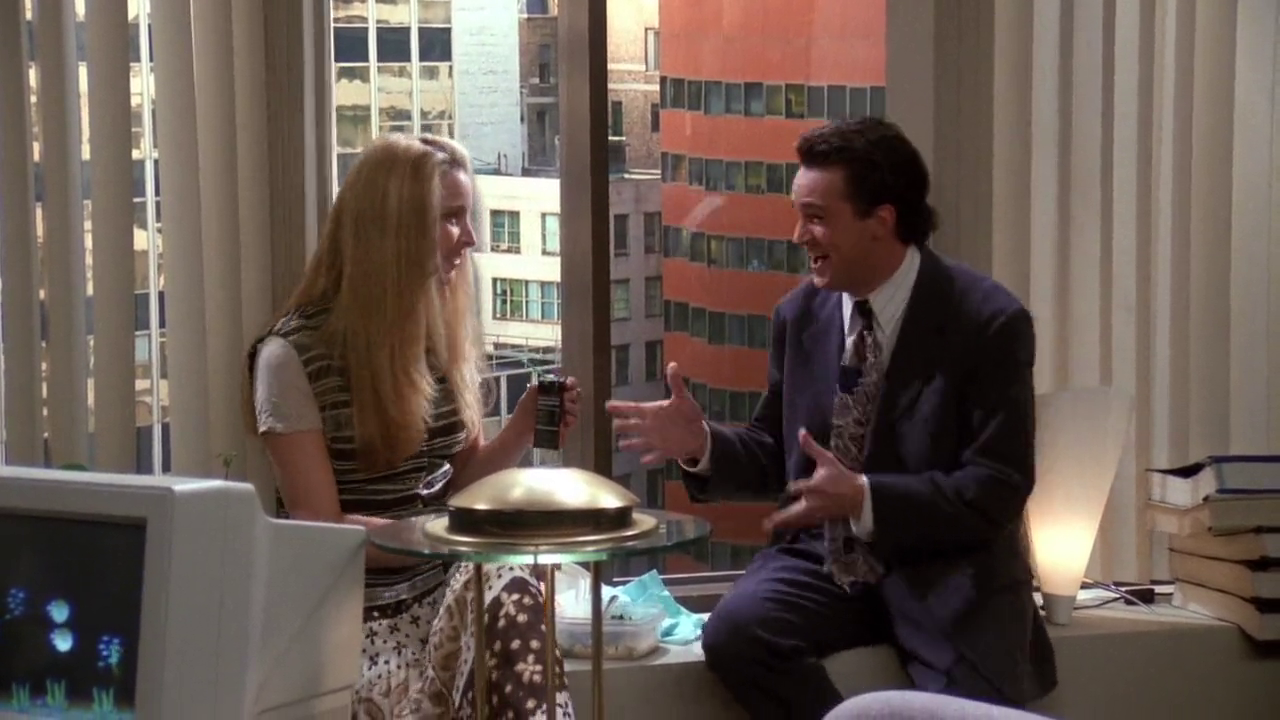
\includegraphics[trim={0 5cm 0 3cm,}, clip, width=\paperwidth]{./S01/img/22/ebony-and-ivory.png}
    % \caption{Ebony and Ivory\label{fig:ebony-and-ivory}}
  \end{adjustwidth}
\end{figure}

\begin{tcolorbox}[enhanced,center upper,
    drop fuzzy shadow southeast, boxrule=0.3pt,
    lower separated=false, breakable,
    colframe=black!30!dialogoBorder,colback=white]
\begin{minipage}[c]{0.16\linewidth}
  \raisebox{\dimexpr-\height+\ht\strutbox\relax}{
    \centering 
\includegraphics[width=1.4cm]{./assets/img/chandler.png}
  }
   & \centering \scriptsize{Chandler}
\end{minipage}
\hfill
\begin{minipage}[c]{0.8\linewidth}
  \textbf{- You know, the karaoke thing? Tracy and I doing Ebony and Ivory?}\\
  - O karaokê foi legal, não é? Tracy e eu cantando Ebony and Ivory?
\end{minipage}
\end{tcolorbox}

Chandler tentava se enturmar na festa do escritório agora que tinha
virado o chefe, e menciona ter cantado a música \emph{Ebony and Ivory}
(1982), um \emph{single} de \emph{Paul McCartney} (1942-) e \emph{Stevie
Wonder} (1950-). A canção é uma alegoria, fazendo paralelo entre as
teclas do piano --- o preto do ébano e o branco do marfim --- e a
integração e harmonia racial. A música aparece no álbum \emph{Tug Of
War} (1982) de \emph{McCartney}.\footnote{\sloppy Paul McCartney - Tug Of War. \url{https://www.paulmccartney.com/albums/tug-of-war}}

\begin{figure}
  \centering
  \begin{tikzpicture}
    \node [inner sep=0pt] at (0,0) {
      
\includegraphics[width=0.5\textwidth,keepaspectratio]{./S01/img/22/tug-of-war.jpg}
    };
    \draw [white, rounded corners=\ClipSep, line width=\ClipSep]
    (current bounding box.north west) --
    (current bounding box.north east) --
    (current bounding box.south east) --
    (current bounding box.south west) -- cycle
    ;
    \end{tikzpicture}
    \caption{Paul McCartney - Tug Of War\label{fig:paul-mc-cartney-tug-of-war}}
\end{figure}
